\documentclass[tikz,dvipdfmx]{standalone}

\usepackage{amsmath, amssymb, amsthm, mathrsfs, amsfonts, dsfont}
\usepackage{mathtools}
\usepackage{ifthen}

\usetikzlibrary{3d,arrows.meta}

\definecolor{cA}{HTML}{0072BD}
\definecolor{cB}{HTML}{EDB120}
\definecolor{cC}{HTML}{77AC30}
\definecolor{cD}{HTML}{D95319}

\begin{document}
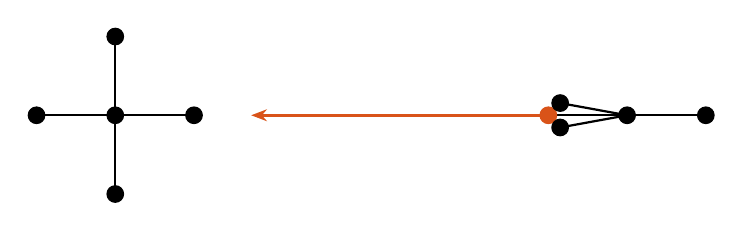
\begin{tikzpicture}
  \foreach \xA/\yA/\xB/\yB/\xC/\yC/\xD/\yD/\xE/\yE/\arrowX/\arrowY/\xShift/\arrowV/\caOne in {
      0/0/-1/0/0/1/0/-1/1/0/0/0/0/a0/black,
      0/0/-1/0/-0.85/0.155/-0.85/-0.155/1/0/-4.77422/0/6.5/a1/cD}{
      \begin{scope}[xshift=\xShift cm]
        \coordinate (a0) at (\xA, \yA);
        \coordinate (a1) at (\xB, \yB);
        \coordinate (a2) at (\xC, \yC);
        \coordinate (a3) at (\xD, \yD);
        \coordinate (a4) at (\xE, \yE);
        \draw[thick] (a0) -- (a1);
        \draw[thick] (a0) -- (a2);
        \draw[thick] (a0) -- (a3);
        \draw[thick] (a0) -- (a4);

        \ifthenelse{\equal{\arrowX}{0} \AND \equal{\arrowY}{0}}{}{
        \draw[-{Stealth[length=2mm]},very thick,cD] (\arrowV) -- (\arrowX, \arrowY);
        }

        \filldraw[draw=black,fill=black] (a0) circle (3pt);
        \filldraw[draw=\caOne,fill=\caOne]   (a1) circle (3pt);
        \filldraw[draw=black,fill=black] (a2) circle (3pt);
        \filldraw[draw=black,fill=black] (a3) circle (3pt);
        \filldraw[draw=black,fill=black] (a4) circle (3pt);
      \end{scope}
    }
\end{tikzpicture}
\end{document}